\chapter{Inleiding}
\label{ch:inleiding}

\section{NoSQL}
Sinds de term in 1998 voor het eerst gebruikt werd door Carlo Strozzi, ging de bal aan het rollen rond NoSQL databanken.
Toen hij deze term de wereld instuurde, , doelde Strozzi met de term op een databank die op dat moment geen SQL interface aanbood.
In 2009 werd de term NoSQL opnieuw gebruikt door Johan Oskarsson als hashtag voor een meetup, waar de problemen met relationele databanken en de huidige manier van programmeren besproken gingen worden.
Nu wordt NoSQL gelezen als 'Not only SQL', wat erop wijst dat er meerdere manieren zijn om data op te slaan. \citep{Fowler2013Introduction}

NoSQL databanken vinden hun oorsprong in de moeilijkheid om objecten uit een object georiënteerd programma op te slaan in een relationele databank: de  zogenoemde 'impedance mismatch', bovendien is er het feit dat relationele databanken vaak niet goed werken op een cluster of niet met grote hoeveelheden realtime data om kunnen gaan\dots
Als gevolg hiervan maken NoSQL databanken vaak geen gebruik van een relationeel model, zijn ze gemaakt om op clusters te werken en zijn ze bovendien schema-less\dots
Kortom databanken onder de noemer NoSQL zijn aangepast om de problemen, die zich nu binnen de relationele databanken manifesteren, aan te pakken \citep{Fowler2012NoSQLDef}.

\cite{Sadalage2014OverviewNoSQL} zegt dat binnen de NoSQL databanken vier grote types naar voor geschoven kunnen worden, namelijk key-value stores (Riak, Redis\dots), document stores (MongoDB, CouchDB\dots), Column Family Stores (Cassandra, HBase\dots) en Graph databases (Neo4J, Infinite Graph\dots).
Elk van deze types heeft zijn eigen specifieke use cases.
Zelfs binnen de verschillende types NoSQL databanken komen er nog verschillende specifieke use cases voor.

Bij gedistribueerde systemen zijn de consistentie, de beschikbaarheid en de partitie tolerantie enorm belangrijk.
\cite{brewer2000towards} stelde hiervoor het CAP theorema op en stelde dat het onmogelijk was om binnen een gedistribueerd systeem deze drie zaken samen te bekomen.
Hij gaf hiermee de aanzet tot de veronderstelling dat er slechts twee van de drie punten in het CAP theorema tegelijk verkregen kunnen worden.
Men is dus genoodzaakt om één eigenschap op te offeren.

Maar wat houden deze drie punten die Brewer aanhaalt nu juist in?

\begin{itemize}
	\item \textbf{Consistency}: De data is op ieder moment op alle nodes gelijk.
	\item \textbf{Availability}: Als een node uitvalt, dan beïnvloedt dit de andere nodes niet.
	\item \textbf{Partition Tolerance}: Het systeem blijft werken ook al zijn er netwerkfouten.
\end{itemize}

\begin{figure}[H]
	\centering
	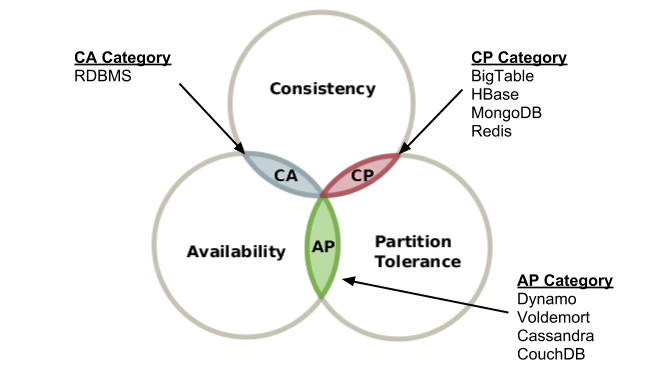
\includegraphics[width=1\textwidth]{img/2_inleiding/cap}
	\caption{CAP theorema \citep{Alvarado2014CAP}}
	\label{fig:cap}
\end{figure}

Als softwareontwikkelaar heeft men keuze uit een hele reeks databanken.
Voor de komst van NoSQL was er echter geen sprake van een keuze.
Lange tijd kon er enkel een relationele database gebruikt worden omdat er niets anders voor handen was.
Wanneer men voor een bepaalde databank kiest is het belangrijk dat men vooraf weet hoe de data gebruikt zal worden.
Wanneer men hier inzicht in heeft, kan men gericht gaan zoeken naar een geschikte databank, hetzij een relationele databank, hetzij een NoSQL databank.

\section{Cassandra}

In het vervolg van deze bachelorproef wordt de focus gelegd op de NoSQL databank Cassandra.
Cassandra is een Column Family database die focust op schaalbaarheid en beschikbaarheid, zonder aan performantie in te boeten.
Cassandra is op dit moment een productiewaardige database.
Enkele bekende gebruikers van Cassandra zijn Facebook, Apple, Netflix, GitHub, Instagram, GoDaddy\dots

Cassandra is een project dat zijn oorsprong vindt bij Facebook.
In 2008 was Cassandra, bedacht door Lakshman en Malik, de oplossing voor het Inbox Search probleem van Facebook.
De moeilijkheid hierbij was dat er een systeem nodig was die eerst en vooral een hoge throughput toelaat, die daarnaast miljarden write operaties per dag moet aankunnen en die bovendien mee kan schalen met het aantal gebruikers \citep{lakshman2010cassandra}.
Om tot deze oplossing te komen baseerden Lakshman en Malik zich op twee andere projecten.

Een eerste project waarop Cassandra gebaseerd is, is Google BigTable.
Google BigTable had namelijk al een oplossing voor een eerste probleem dat Lakshman en Malik moesten oplossen: een schaalbare database die ook realtime antwoorden toelaat \citep{chang2008bigtable}.
Lakshmans vorige project, Amazon Dynamo, was de tweede inspiratiebron voor Cassandra.
Dynamo zorgde eerder al voor een hoge betrouwbaarheid bij een schaalbare database \citep{decandia2007dynamo}.

Hoewel Cassandra niet verder uitgebreid moest worden omdat het nog steeds voldeed aan de voorwaarden om het probleem van Facebook op te lossen, is Cassandra verder blijven groeien sinds 2008.
Zo kan Cassandra nu bijvoorbeeld ook overweg met gestructureerde, semi-gestructureerde en ongestructureerde data \citep{kan2014cassandra}.

Als men Cassandra binnen het CAP theorema moet gaan classificeren, kan men stellen dat de focus hier ligt op beschikbaarheid en partitie tolerantie.
Binnen Cassandra kan er toch een keuze gemaakt worden tussen snelheid en consistentie.
Hiermee kan een zeer hoge consistentie en ook een aanvaardbare snelheid verkregen worden \citep{ellis2009cassandra}.
Met het oorspronkelijk CAP theorema is dit echter niet mogelijk.
\cite{brewer2012cap} herformuleerde echter het CAP theorema omdat hij vond dat het twee-uit-drie-concept misleidend was.
Hier stelde hij dat een keuze voor de drie mogelijkheden mogelijk was als er goed nagedacht werd over de partities.

\section{Probleemstelling en onderzoeksvragen}
\label{sec:onderzoeksvragen}

% TODO: Wees zo concreet mogelijk bij het formuleren van je
% onderzoeksvra(a)g(en). Een onderzoeksvraag is trouwens iets waar nog
% niemand op dit moment een antwoord heeft (voor zover je kan nagaan).

Cassandra belooft een groot aantal zaken en binnen deze bachelorproef is het de bedoeling om deze beloften na te gaan.
Eerst en vooral zal de schaalbaarheid van Cassandra gecontroleerd worden.
Is het werkelijk eenvoudig om de database op verschillende eenvoudige servers te installeren?
Een tweede punt dat nagegaan wordt is de betrouwbaarheid van Cassandra.
Is er werkelijk geen ''single point of failure'' en in hoeverre zijn back-ups nodig binnen deze NoSQL omgeving?
Een laatste punt waarbij er stilgestaan wordt, is de data modellering in Cassandra.